\chapter{Pruebas y resultados} \label{cap:pruebas_y_resultados}
% Breve descripción del capítulo
El capítulo de pruebas y resultados como su nombre lo indica pretende observar el desempeño del sistema de navegación en diferentes situaciones para interpretar los resultados obtenidos. Al comienzo de este capítulo, en la sección \ref{sec:integración_mediante_la_plataforma_ROS} se describen de forma breve todos y cada uno de los nodos desarrollados para el sistema de navegación. En las posteriores secciones \ref{sec:pruebas_de_navegación_sin_obstáculos}, \ref{sec:pruebas_de _navegación_con_obstáculos} y \ref{sec:pruebas_de_navegación_con_obstáculos_en_movimiento} se exponen las pruebas para navegación sin obstáculos, navegación con obstáculos y navegación con obstáculos en movimiento respectivamente. En cada una de estas secciones se menciona qué se busca comprobar además de mencionar las condiciones que son requeridas, finalmente se exponen los resultados obtenidos durante cada prueba.

\section{Integración mediante la plataforma ROS} \label{sec:integración_mediante_la_plataforma_ROS}

El sistema navegación del vehículo autónomo es logrado a través de una combinación de diferentes tecnologías. Como se mencionó en capítulos anteriores Webots es el simulador utilizado para modelar los escenarios, vehículos de obstáculo y el propio vehículo autónomo. Los controladores y supervisores que utilizan los elementos modelados en el simulador fueron desarrollados con el lenguaje de programación Python. Por otro lado, los nodos que conforman al sistema de navegación fueron desarrollados en su mayoría con Python y otros más con C++, finalmente, la parte de comunicación por mensajes entre nodos es con la plataforma ROS.

A continuación se describen brevemente cada uno de los nodos que forman parte del sistema de navegación del vehículo.

\hfill

\textbf{\textit{ros\_car\_controller}}
\begin{itemize}
    \item \textbf{Descripción:} Nodo responsable de obtener y comunicar la información de los sensores(Cámara y LIDAR), así como el ángulo de dirección actual del vehículo autónomo. Además, sitúa los valores de velocidad y ángulo de dirección en los actuadores correspondientes del vehículo autónomo.
    \item \textbf{Tópicos publicados:} 
    \begin{itemize}
        \item /current\_steering
        \item /camera/rgb/raw
        \item /point\_cloud
    \end{itemize}
    \item \textbf{Tópicos suscritos:}
    \begin{itemize}
        \item /goal\_speed
        \item /goal\_steering
    \end{itemize}
\end{itemize}
\hfill

\textbf{\textit{lane\_detect}}
\begin{itemize}
    \item \textbf{Descripción:} Este nodo tiene la finalidad de procesar una imagen RGB que proviene de la cámara del vehículo para hacer la detección de carril, hace uso de las herramientas de detector de bordes de Canny y detección de líneas rectas con transformada Hough explicadas en el capítulo \ref{cap:seguimiento_de_carriles}. El resultado de la ejecución de este nodo son dos líneas rectas en forma polar que corresponden a los bordes del carril identificado.
    \item \textbf{Tópicos publicados:}
    \begin{itemize}
        \item /left\_lane
        \item /right\_lane
    \end{itemize}
    \item \textbf{Tópicos suscritos:} 
\begin{itemize}
    \item /camera/rgb/raw
\end{itemize}
\end{itemize}
\hfill

\textbf{\textit{object\_detect}}
\begin{itemize}
    \item \textbf{Descripción:} Nodo responsable de obtener la nube de puntos del sensor LIDAR, filtrarla y agruparla con el algoritmo \textit{k-means}. La salida de este nodo es un conjunto de centroides que representan la posición media de los obstáculos detectados.
    \item \textbf{Tópicos publicados:}
    \begin{itemize}
        \item /object\_pose
    \end{itemize}
    \item \textbf{Tópicos suscritos:}
    \begin{itemize}
        \item /point\_cloud
    \end{itemize}
\end{itemize}

\newpage

\textbf{\textit{object\_tracking}}
\begin{itemize}
    \item \textbf{Descripción:} Este nodo se encarga de empatar y estimar posición y velocidad de los obstáculos detectados con el algoritmo \textit{k-means}. Para el empatado utiliza el algoritmo \ref{alg:matching} y para la estimación el filtro de Kalman diseñado en la sección \ref{sub:estimación_de_posición_y_velocidad_con_el_filtro_de_kalman_extendido} del capítulo \ref{cap:detección_de_obstáculos}. Como resultado de este proceso se obtiene un conjunto de pares [obstáculo, EKF], donde ``obstáculo'' es un identificador para cada obstáculo detectado y ``EKF'' es su correspondiente filtro de Kalman con posición y velocidad estimadas.
    \item \textbf{Tópicos publicados:} 
    \begin{itemize}
        \item /filter\_pose
    \end{itemize}
    \item \textbf{Tópicos suscritos:}
    \begin{itemize}
        \item /object\_pose
    \end{itemize}
\end{itemize}
\hfill

\textbf{\textit{object\_avoidance}}
\begin{itemize}
    \item \textbf{Descripción:} El sistema de árbitro explicado en el capítulo \ref{cap:comportamientos} es representado por este nodo. Define el conjunto de zonas ocupadas utilizando las posiciones estimadas con el EKF, implementa la máquina de estados de la figura \ref{fig:main_sm} y comunica las señales de habilitación para los comportamientos de crucero, mantener distancia y rebase. También, para el comportamiento de mantener distancia, calcula y comunica la distancia que existe entre el vehículo autónomo y el coche de enfrente, en el caso del comportamiento rebase, recibe una señal que indica cuando se ha completado esta acción.
    \item \textbf{Tópicos publicados:} 
    \begin{itemize}
        \item /enable\_LT
        \item /enable\_KD
        \item /enable\_PS
        \item /safe\_distance
    \end{itemize}
    \item \textbf{Tópicos suscritos:}
    \begin{itemize}
        \item /filter\_pose
        \item /pass\_finished
    \end{itemize}
\end{itemize}

\newpage
\textbf{\textit{lane\_tracking}}
\begin{itemize}
    \item \textbf{Descripción:} Este nodo representa al comportamiento de crucero y su objetivo es implementar las leyes de control vistas en el capítulo \ref{cap:seguimiento_de_carriles} para las funciones tácticas de movimiento lateral y longitudinal del vehículo (ángulo de dirección y velocidad). Hace uso de los bordes de carril detectados con el nodo /lane\_detect y cuenta con una señal de habilitación proveniente del árbitro para activarse o desactivarse.
    \item \textbf{Tópicos publicados:}
    \begin{itemize}
        \item /goal\_speed
        \item /goal\_steering
    \end{itemize}
    \item \textbf{Tópicos suscritos:}
    \begin{itemize}
        \item /left\_lane
        \item /right\_lane
        \item /enable\_LT
    \end{itemize}
\end{itemize}
\hfill

\textbf{\textit{keep\_distance}}
\begin{itemize}
    \item \textbf{Descripción:} Este nodo reproduce al comportamiento de mantener distancia. Calcula la ley de control para velocidad del vehículo con la ecuación (\ref{eqn:keep_distance_velocity}) explicada en la sección \ref{sub:mantener_distancia} mientras que el ángulo de dirección es de la misma forma que en el comportamiento de crucero, se utiliza el detector y seguidor de carril del capítulo \ref{cap:seguimiento_de_carriles}. Recibe por parte del nodo /object\_avoidance un habilitador de comportamiento y una distancia que es utilizada en el cálculo de velocidad.
    \item \textbf{Tópicos publicados:}
    \begin{itemize}
        \item /goal\_speed
        \item /goal\_steering
    \end{itemize}
    \item \textbf{Tópicos suscritos:}
    \begin{itemize}
        \item /safe\_distance
        \item /left\_lane
        \item /right\_lane
        \item /enable\_KD
    \end{itemize}
\end{itemize}

\newpage

\textbf{\textit{overtake}}
\begin{itemize}
    \item \textbf{Descripción:} Este nodo se encarga de representar al comportamiento de rebase, implementa la máquina de estados vista en la imagen \ref{fig:pass_sm} para lograrlo. Calcula las leyes de control mostradas en la sección \ref{sub:rebase} para el movimiento del vehículo en este comportamiento. Al igual que los comportamientos de crucero y mantener distancia, recibe un habilitador para activarse o desactivarse según corresponda, finalmente, envía una señal al árbitro para indicar cuando se ha terminado una acción de rebase.
    \item \textbf{Tópicos publicados:}
    \begin{itemize}
        \item /goal\_speed
        \item /goal\_steering
        \item /pass\_finished
    \end{itemize}
    \item \textbf{Tópicos suscritos:}
    \begin{itemize}
        \item /enable\_PS
        \item /current\_steering
    \end{itemize}
\end{itemize}
\hfill

En la figura \ref{fig:nodes} se pueden observar cada uno de los nodos del sistema de navegación previamente descritos. Ahí, se pueden apreciar los tópicos a los que se suscribe cada nodo así como los tópicos publicados por cada uno.
\begin{figure}[h]
    \centering
    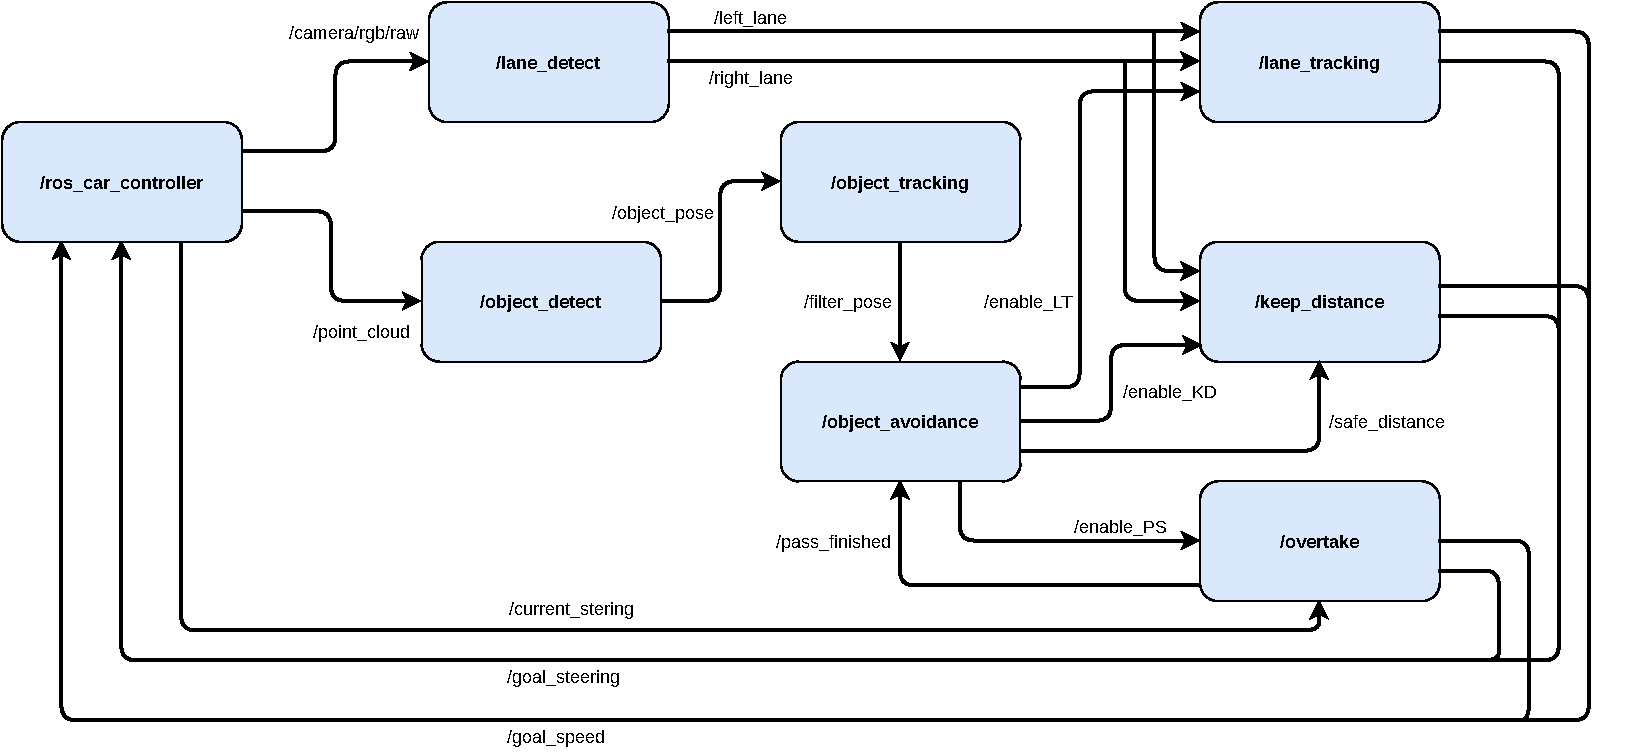
\includegraphics[width=1.0\textwidth]{Figures/Figures_Cap07/nodes.pdf}
    \caption{Nodos del sistema de navegación. Los rectángulos color azul representan a los nodos y las flechas es la comunicación entre nodos mediante tópicos.}
    \label{fig:nodes}
\end{figure}

% \textcolor{red}{
% \begin{itemize}
%   \item Descripción de cada nodo con los tópicos publicados/suscritos y servicios requeridos/atendidos
% \end{itemize}
% }
\newpage
Los nodos descritos anteriormente forman la arquitectura de autonomía de sistema de navegación del vehículo no tripulado de este trabajo. Esta arquitectura cuenta con dos principales sistemas: percepción y decisión. En la figura 4, se muestra a que sistema pertenece cada nodo desarrollado.
\begin{figure}[h]
    \centering
    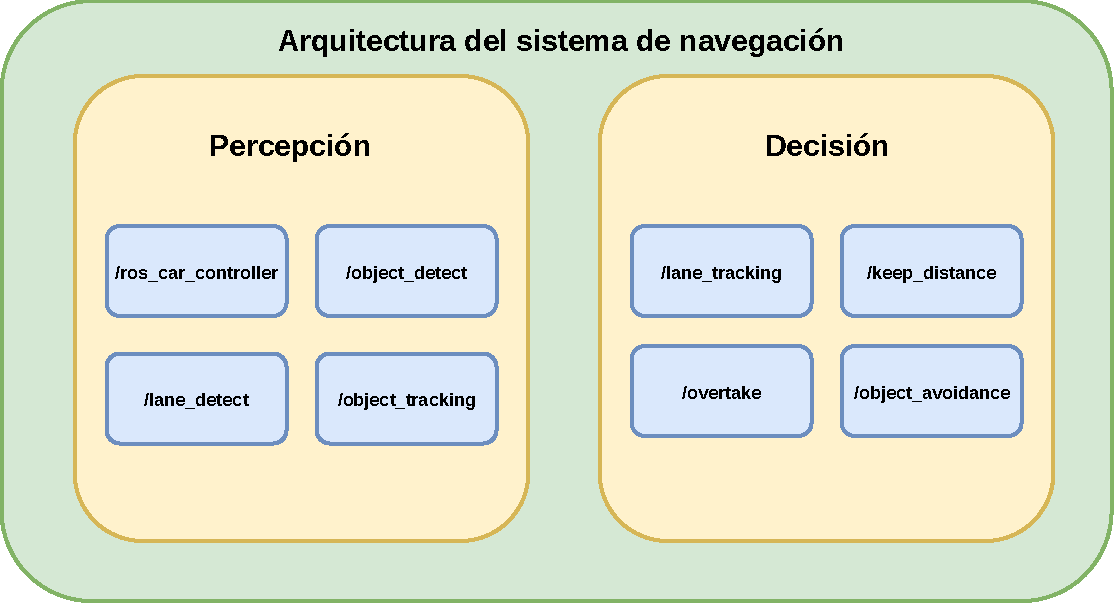
\includegraphics[width=0.75\textwidth]{Figures/Figures_Cap07/architecture.pdf}
    \caption{Arquitectura del sistema de navegación.}
    \label{fig:architecture}
\end{figure}

Antes de mencionar los resultados obtenidos en las diferentes pruebas es importante mencionar que el circuito de pruebas es el que se mencionó en el capítulo \ref{cap:simulación_con_webots} en la figura \ref{fig:webots_world}. En cada una de las pruebas se modificó el mundo creado para añadir elementos o modificar características de los obstáculos.

\section{Pruebas de navegación sin obstáculos} \label{sec:pruebas_de_navegación_sin_obstáculos}

La prueba de navegación sin obstáculos tiene la finalidad de verificar el comportamiento de ``Crucero''. Para esta prueba el vehículo autónomo debe completar en su totalidad el circuito sin salir de su carril y sin chocar con los bordes del mismo, en este escenario no existen obstáculos en la carretera, la figura \ref{fig:navigation_no_obstacles} muestra el circuito para esta prueba.
\begin{figure}[h]
    \centering
    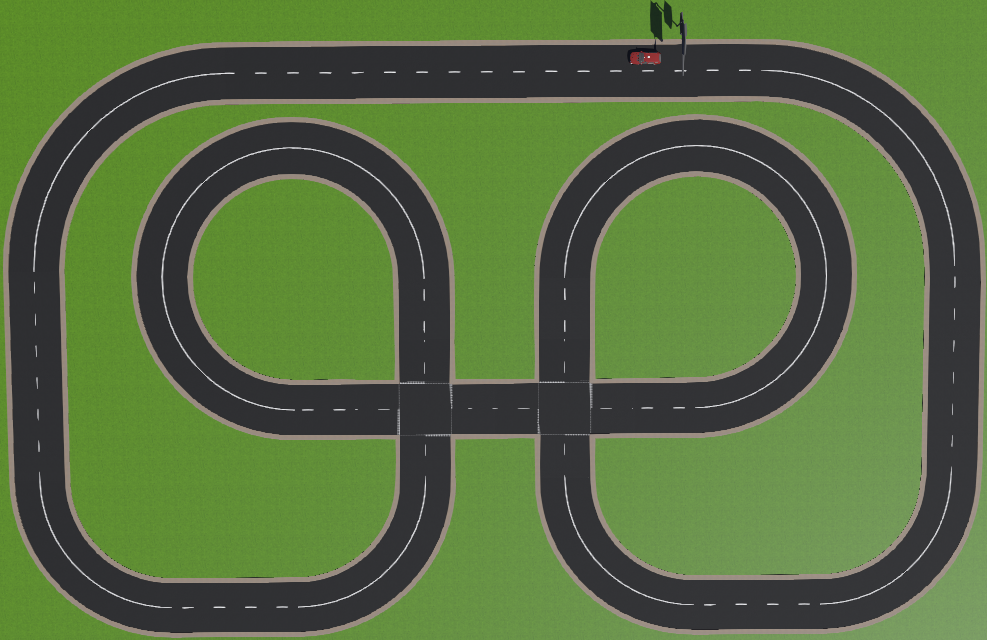
\includegraphics[width=0.5\textwidth]{Figures/Figures_Cap07/navigation_no_obstacles.png}
    \caption{Circuito de pruebas para navegación sin obstáculos.}
    \label{fig:navigation_no_obstacles}
\end{figure}

Como ya se ha mencionado, la velocidad $v$ del vehículo en el comportamiento de ``Crucero'' es constante en todo momento, la documentación de Webots indica que la velocidad del vehículo es en unidades de km/h. Teniendo esto en cuenta, se realizaron diferentes experimentos para este comportamiento con diferentes velocidades con el fin de observar y comprobar el desempeño de la conducción del vehículo. La siguiente tabla muestra algunas de las velocidades que se probaron.
\begin{table}[h]
    \begin{center}
        \begin{tabular}{c|l}
        \hline
            Velocidad [km/h] & Observación\\ \hline 
            30.0 & Completó el circuito correctamente.\\ 
            35.0 & Completó el circuito correctamente.\\
            40.0 & Completó el circuito correctamente.\\ 
            45.0 & Salió del carril en curvas.\\ 
            50.0 & El vehículo se volteó en curvas.\\ 
            55.0 & El vehículo no giró en curvas y salió del circuito.\\
            60.0 & El vehículo no giró en curvas y salió del circuito.
        \end{tabular}
    \end{center}
    \caption{Pruebas de velocidad para navegación sin obstáculos.}
    \label{tab:navigation_no_obstacles}
\end{table}
En la tabla \ref{tab:navigation_no_obstacles} se puede observar que conforme aumenta la velocidad del vehículo el control del ángulo de dirección es inestable. Esto es provocado por el error que existe entre los bordes de carril observados y originales, como consecuencia se obtienen cambios pequeños o muy grandes en el ángulo de dirección. En casos extremos cuando la velocidad $v$ fue $> 50$ km/h el vehículo logró mantenerse en su carril en caminos rectos pero no logró girar en curvas. Con velocidades en el rango de $[40.0-50.0]$ km/h el vehículo se mantuvo en su carril en rectas pero en curvas a la izquierda o derecha se volteó por completo. Sin embargo, cuando la velocidad varió entre 30 y 40 km/h, el vehículo se comportó de muy buena forma, realizó giros suaves en curvas y se mantuvo bien alineado dentro de su carril en todo momento. En este rango de velocidades el vehículo logró completar el circuito en su totalidad sin salir de su carril y por su puesto sin chocar con los bordes del carril.

Con estos resultados se optó por mantener la velocidad en el rango de $[30.0-40.0]$ km/h para esta y las siguientes pruebas.

\section{Pruebas de navegación con obstáculos} \label{sec:pruebas_de _navegación_con_obstáculos}

Para las pruebas de navegación con obstáculos sin movimiento se añadieron vehículos en diferentes posiciones del circuito pero en el mismo carril que el vehículo autónomo, la modificación al mundo es mostrado en la figura \ref{fig:navigation_static_obstacles}. En este escenario se busca probar el comportamiento de ``Crucero'' mientras no existan vehículos que impidan el camino del vehículo autónomo, cuando esto suceda se pondrá aprueba el comportamiento de ``Rebase'', el cual debe de realizarse sin chocar y sin salir del circuito.
\begin{figure}[h]
    \centering
    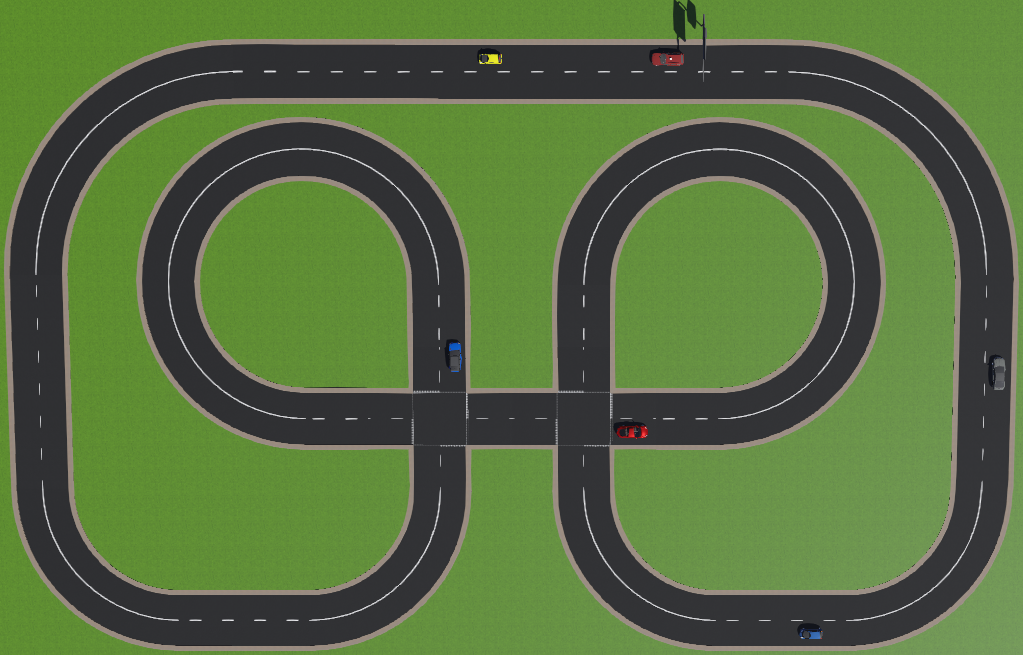
\includegraphics[width=0.5\textwidth]{Figures/Figures_Cap07/navigation_static_obstacles.png}
    \caption{Circuito de pruebas para navegación con obstáculos estáticos.}
    \label{fig:navigation_static_obstacles}
\end{figure}

Debido a los resultados obtenidos en las pruebas de navegación sin obstáculos se concluyó que la velocidad que ofrece mayor seguridad es de 30.0 km/h en el comportamiento de ``Crucero''. Para mantener la seguridad del vehículo autónomo durante una acción de rebase se optó por tener una velocidad constante de 20.0 km/h durante este comportamiento. 

En la imagen \ref{fig:navigation_static_obstacles} se observa que hay en total 5 vehículos como obstáculos. Para la prueba de navegación con obstáculos estáticos se realizaron 10 simulaciones de manera consecutiva, en la siguiente tabla se muestran los resultados con la cantidad de rebases bien hechos por el vehículo autónomo en cada simulación:
\begin{table}[h]
    \begin{center}
        \begin{tabular}{c|c}
        \hline
            Simulación & Cantidad de rebases bien realizados\\ \hline 
            1 & 2 \\ 
            2 & 3\\ 
            3 & 5\\ 
            4 & 0\\ 
            5 & 3\\ 
            6 & 4\\ 
            7 & 5\\ 
            8 & 5\\ 
            9 & 0\\ 
            10 & 4\\ 
        \end{tabular}
    \end{center}
    \caption{Pruebas de rebase para navegación con obstáculos estáticos.}
    \label{tab:navigation_static_obstacles}
\end{table}

Con los resultados de la tabla \ref{tab:navigation_static_obstacles} se entiende que en un $30\%$ de las simulaciones se completó el circuito realizando de manera correcta los rebases, en $20\%$ de las ocasiones se lograron 4 rebases que equivale a recorrer $3/4$ del circuito, otro $20\%$ de las ocasiones indica que solo se realizaron 3 rebases, es decir, recorrió poco más de la mitad del circuito. Los casos más extremos se presentaron cuando solo se realizaron dos rebases ($10\%$) y ningún rebase ($20\%$). 

Como se mencionó en la sección \ref{sub:rebase}, el comportamiento de ``Rebase'' se realiza en lazo abierto. Dicho de otro modo, todas las situaciones de rebase que detecte el vehículo se realizarán de la misma forma, sin ningún tipo de retroalimentación. Esto tiene como consecuencia que el vehículo no logré completar un rebase en algunas ocasiones. Sin embargo, durante estas simulaciones se verifica el buen funcionamiento del sistema de árbitro porque se nota el cambio entre comportamientos, el comportamiento de ``Crucero'' funciona correctamente antes y después de una acción de rebase. En el caso del comportamiento ``Rebase'' ya se han mencionado los resultados obtenidos.

\section{Pruebas de navegación con obstáculos en movimiento} \label{sec:pruebas_de_navegación_con_obstáculos_en_movimiento}

Las pruebas de navegación con obstáculos en movimiento tiene dos propósitos principales. Primero, observar el desempeño del comportamiento de ``Rebase'' cuando el vehículo por rebasar se encuentre en movimiento. El segundo objetivo es verificar el comportamiento de ``Mantener distancia'' cuando se presente una posible situación de tráfico. Para estos dos propósitos se realizaron algunas modificaciones a los escenarios previos.

Para el comportamiento de ``Rebase'' se mantuvo la misma cantidad de obstáculos en el circuito, a diferencia del circuito de la figura \ref{fig:navigation_static_obstacles} donde el primer vehículo (en color amarillo) se mantiene estático ahora se puede desplazar de forma longitudinal. Para ello, se le asigna una velocidad constante para avanzar hacia adelante, la velocidad de este coche es más pequeña que la velocidad de rebase del vehículo autónomo. Tanto la velocidad como el tiempo que dura el movimiento del vehículo amarillo son manipulados a través de un controlador supervisor. El resto de los vehículos en el circuito se mantienen estáticos pero en diferentes posiciones, en \ref{fig:navigation_dynamic_obstacles} se muestra el escenario para esta prueba de navegación.
\begin{figure}[h]
    \centering
    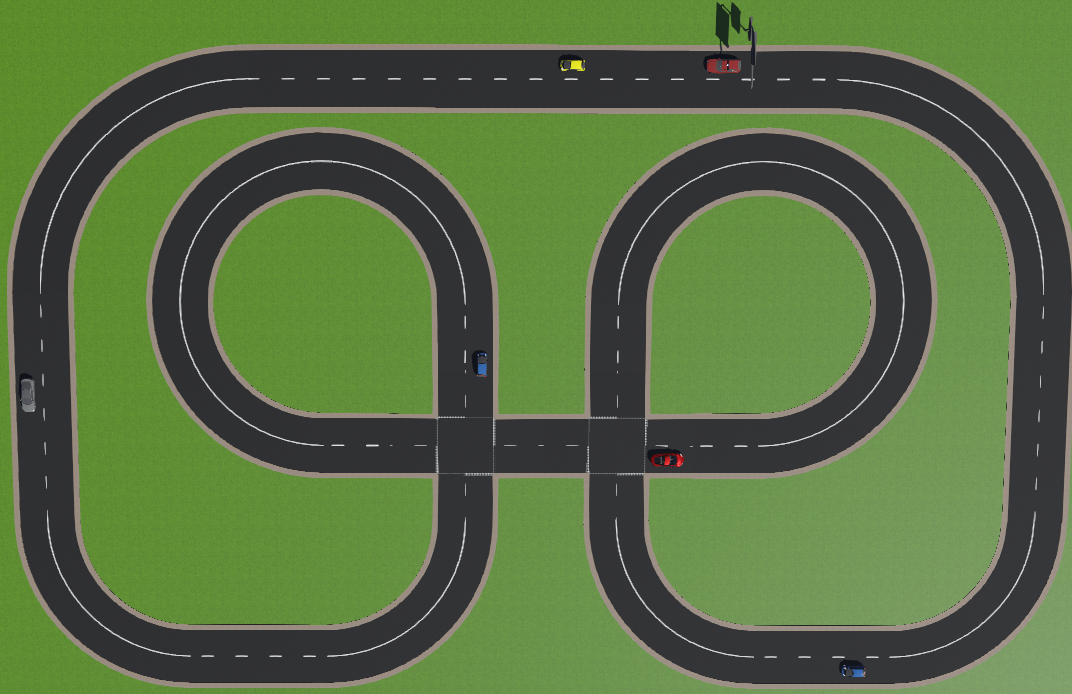
\includegraphics[width=0.5\textwidth]{Figures/Figures_Cap07/navigation_dynamic_obstacles.png}
    \caption{Circuito de pruebas para navegación con obstáculos en movimiento.}
    \label{fig:navigation_dynamic_obstacles}
\end{figure}

Al igual que en las pruebas de navegación con obstáculos estáticos se realizaron 10 simulaciones consecutivas para navegación con obstáculos dinámicos. En la tabla \ref{tab:navigation_dynamic_obstacles} se muestran los resultados de la acción realizada por el vehículo autónomo solo para el primer rebase, porque este vehículo es el que tiene movimiento.
\begin{table}[h]
    \begin{center}
        \begin{tabular}{c|l}
        \hline
            Simulación & Observación del vehículo autónomo\\ \hline 
            1 & Realizó el rebase correctamente.\\ 
            2 & Realizó el rebase pero choca al costado.\\ 
            3 & Realizó el rebase correctamente.\\ 
            4 & Realizó el rebase correctamente.\\ 
            5 & No realizó rebase.\\ 
            6 & Realizó el rebase pero choca al costado.\\ 
            7 & Realizó el rebase correctamente.\\ 
            8 & Realizó el rebase correctamente.\\ 
            9 & No realizó rebase.\\ 
            10 & Realizó el rebase correctamente.\\ 
        \end{tabular}
    \end{center}
    \caption{Pruebas de rebase para navegación con obstáculos dinámicos.}
    \label{tab:navigation_dynamic_obstacles}
\end{table}

Como lo indica la tabla anterior en el $60\%$ de las simulaciones el vehículo autónomo logró realizar el rebase correctamente, solo en dos ocasiones $(20\%)$ se realizó el rebase pero con un ligero choque al costado, lo cual no es correcto y en el otro $20\%$ no se logró realizar el rebase.

La segunda adecuación tiene que ver con el comportamiento de ``Mantener distancia''. Retomando el circuito anterior, a este circuito se añadió un vehículo más que se encuentra en el carril izquierdo, ver \ref{fig:navigation_keep_distance}. La posición de estos vehículos simulan una posible situación de tráfico como las propuestas en la imagen \ref{fig:obstacle_zones}. A estos dos vehículos también se les asignaron velocidades constantes para que puedan desplazarse hacia adelante, el movimiento inicia al comienzo de la simulación.
\begin{figure}[h]
    \centering
    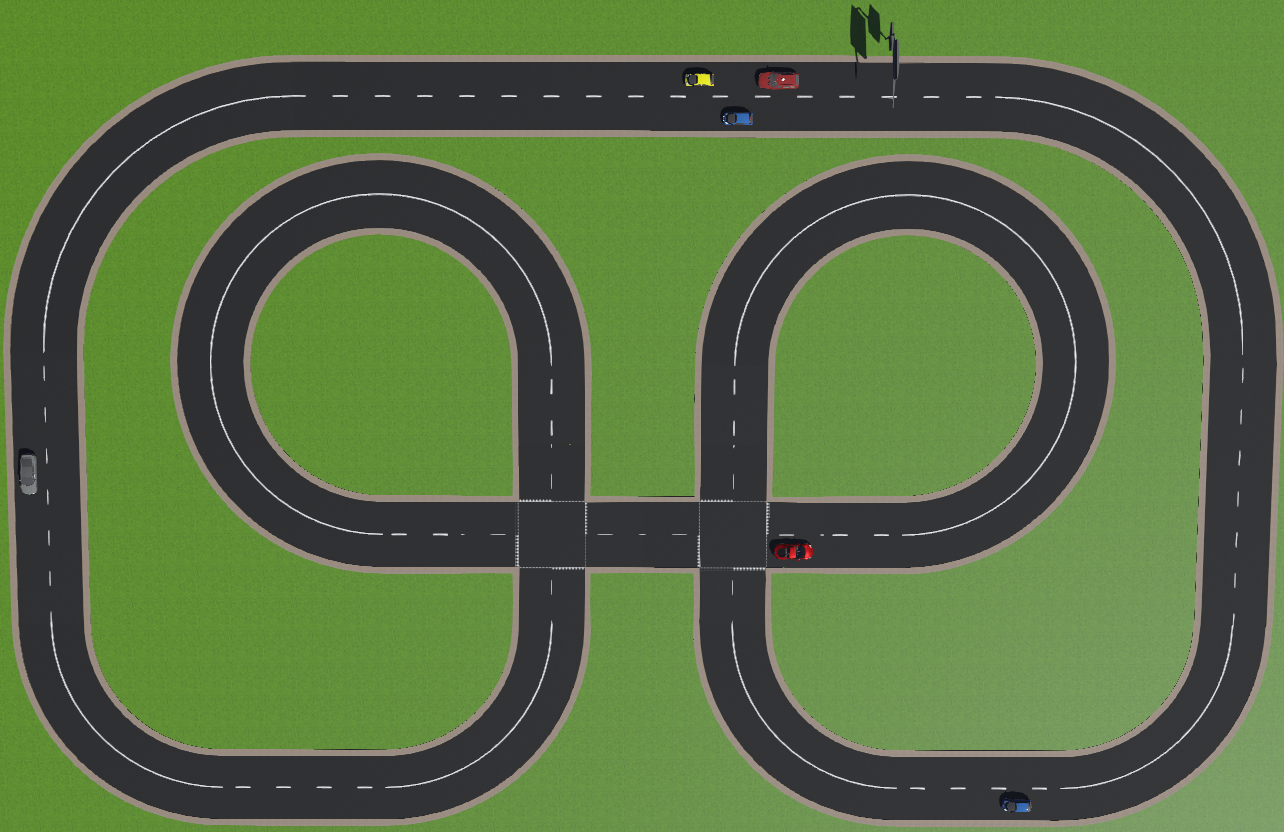
\includegraphics[width=0.5\textwidth]{Figures/Figures_Cap07/navigation_keep_distance.png}
    \caption{Circuito de pruebas para navegación con obstáculos en movimiento (Mantener distancia).}
    \label{fig:navigation_keep_distance}
\end{figure}

Para la prueba de este comportamiento también se ejecutaron 10 simulaciones de manera continúa, en todas estas simulaciones el vehículo autónomo detectó el comportamiento de ``Mantener distancia'' y por lo tanto reguló la velocidad original logrando mantenerse a una distancia segura de los vehículos (amarillo y azul) y por ello evitar percances. 

% CONCLUSIONES DEL CAPÍTULO
Con el conjunto de pruebas realizadas para la navegación del vehículo autónomo en un circuito cerrado sin obstáculos y con obstáculos tanto estáticos como en movimiento se logró observar el desempeño de los comportamientos de ``Crucero'', ``Rebase'' y ``Mantener distancia'' además del árbitro para la elección de estos. Durante estas pruebas los resultados indicaron que se puede completar el circuito propuesto manteniendo situaciones controladas, en el caso de navegación sin obstáculos solo se requirió que fueran visibles las líneas que delimitan el carril y obviamente no existan obstáculos en el camino. El rebase se comprobó con las pruebas de navegación con obstáculos con y sin movimiento, el desempeño de este comportamiento fue positivo en más de la mitad de las ocasiones que fue requerido. Sin embargo, en algunas ocasiones el balance no fue satisfactorio por razones anteriormente expresadas. Finalmente y en específico con la prueba de navegación con obstáculos en movimiento se logró observar el funcionamiento del comportamiento ``Mantener distancia'', el cual fue exitoso en las simulaciones realizadas. 

Estas pruebas también permitieron verificar el funcionamiento de todos los nodos creados, trabajando y comunicándose en conjunto mediante la plataforma ROS además de los controladores desarrollados para algunos elementos presentes en las simulaciones. Como resultado de esto se puede afirmar que el sistema de navegación del vehículo autónomo funciona adecuadamente siempre y cuando se encuentran en escenarios y con condiciones controladas como los vistas a lo largo de este trabajo. En el siguiente capítulo se abordarán conclusiones más específicas en los resultados obtenidos durante todo el desarrollo. También, se mencionarán posibles mejoras por implementar en el sistema de navegación en la búsqueda de obtener mejores resultados.

Cabe mencionar que este es un proyecto de código abierto y por lo tanto, se encuentra libre, en específico, dentro de un repositorio de la plataforma GitHub \footnote{\url{https://github.com/Davidtrejo590/Webots-ROS}}. Dentro del repositorio se incluyen los códigos fuente de cada nodo, mundos creados en el simulador Webots para las pruebas de navegación así como los controladores y supervisores para el vehículo autónomo y obstáculos. También se incorporan las instrucciones y requisitos necesarios para ejecutar el proyecto completo.

